%
% Adapted from the NAACL-HLT 2016 LaTeX template.
%

\documentclass[11pt,letterpaper]{article}
\usepackage{naaclhlt2016}
\usepackage{times}
\usepackage{latexsym}
\usepackage{graphicx}
\usepackage{subfigure}
\usepackage{balance}
\usepackage{hyperref}
\usepackage{natbib}
\usepackage{arydshln}
\usepackage{enumitem}
\usepackage{booktabs}
\usepackage{tabularx}
\usepackage{longtable}
\usepackage{pdflscape}
\usepackage{array}
\usepackage{float}
\usepackage[table]{xcolor}

\naaclfinalcopy

\newcommand\BibTeX{B{\sc ib}\TeX}

\title{Flagging Potential Research Fraud in Biomedical Papers Using Linguistic Features and Machine Learning}

\author{Brian Wei \\
        Institute for Computing in Research \\
        {\tt brianwei.us@gmail.com}}

\date{}

\begin{document}

\maketitle

\begin{abstract}
Research fraud can remain undetected for years, allowing unreliable findings to influence later research and consume limited grant funding. This study examined whether linguistic features and machine learning could distinguish biomedical papers later retracted for the fabrication, falsification, or manipulation of data or images from matched control papers. A dataset of 1,412 full-text papers was analyzed using extracted linguistic features, biomedical text embeddings, and four machine learning classifiers. Retracted papers showed measurable differences in grammatical structure, repetition, passive voice, and other linguistic characteristics. The best-performing model combined the extracted features and embeddings, achieving 76.4\% total accuracy. These results suggest that linguistic analysis may help flag papers for additional review.
\end{abstract}

\section{Introduction}

The sharp rise in scientific retractions in recent years \cite{citation_needed_retraction_growth}, with a majority of retractions being attributed to misconduct \cite{citation_needed_misconduct_share}, has intensified concerns about fraud and other forms of research misconduct. Research and publication misconduct takes diverse forms, including fabricating data, falsifying results, manipulating images, plagiarizing others' work, and faking peer review. This becomes even more problematic given the alarmingly rapid rise in paper mills---commercial organizations that create and sell fraudulent research---with a recent estimate suggesting that at least 400,000 paper-mill articles have entered the scientific literature \cite{paper_mills_estimate}. This, combined with the replication crisis, which primarily focuses on psychology and biomedical research \cite{openscience2015,begley2012}, as well as the rampant ``publish or perish'' culture, makes research fabrication and fraud extremely necessary to investigate.

\subsection{Consequences of Fabrication and Fraud}

Research misconduct is especially prevalent in biomedical research, occurring much more frequently than in other fields \cite{citation_needed_biomedical_prevalence}. This is especially troublesome because erroneous findings may influence later research, public policy, and public trust. A prominent example is Andrew Wakefield's 1998 study linking the MMR vaccine to autism using falsified data. This sparked an international anti-vaccine movement, and the loss of trust in the vaccine contributed to outbreaks of measles and mumps, leading to many preventable deaths \cite{citation_needed_wakefield_consequences}. The broader damage to vaccine confidence persists today, as seen in hesitancy to adopt the COVID-19 vaccine despite the global pandemic.

Unfortunately, retracting a paper is not enough. The retraction process is very slow, often involving formal investigations that take months or even years, with a median of 2.4 years from publication to retraction for papers involving misconduct \cite{retraction_delay}. Wakefield's 1998 paper was not retracted until 2010, twelve years later. This slow pace allows the research to be incorporated into other works and to influence the general public. A journal simply issuing a retraction notice also does not remove the paper from academia, because retracted papers continue to persist in databases and reference lists. This allows them to continue to be cited after retraction, with approximately 35\% of papers still receiving citations after retraction \cite{post_retraction_citations}. Of these citations, only 5.4\% acknowledge that the cited material was retracted. Allowing these papers to persist within academia harms science as a whole, as future research may continue to build on flawed findings.

There is also a considerable financial cost to fabricated or fraudulent research, as research consumes substantial amounts of public and institutional funding. Grant money for biomedical research, with the taxpayer-funded NIH providing the majority globally, is wasted on these papers. Each fraudulent paper costs, on average, \$400,000 in grant money \cite{misconduct_grant_cost} and another \$500,000 for an institutional investigation \cite{misconduct_investigation_cost}. There are even more indirect costs from other researchers attempting to replicate the results. A conservative estimate from 2010 places the cost at \$110 million annually \cite{misconduct_investigation_cost}, an estimate that is likely higher today due to the increase in retracted papers and total papers written.

\subsection{The Need for Screening}

The peer review process is meant to act as a quality-control process before publication. Peer reviewers are unpaid volunteers working with very limited time. Often, they are limited to only the information in the manuscript and are rarely provided access to raw data, original image files, lab notebooks, or analysis code \cite{peer_review_materials}. This process places a substantial burden on peer reviewers, who volunteer time that could otherwise be spent conducting research. The increasing burden associated with detecting fraud reduces their time for research and may affect their careers. Thus, they simply do not have the resources to perform a forensic audit. Instead, their role is to evaluate the scientific rigor of the methods, analyses, and conclusions, as well as the quality of the presentation.

Consequently, it may be easy for fabricated data, duplicated images, or paper-mill manuscripts to survive the peer review process. The reviewers are not negligent, but they simply lack the time, underlying materials, specialized tools, and expertise required to screen for integrity. Computational methods could assist peer reviewers by helping flag papers for additional review. This would avoid wasting time auditing every paper while also preventing potentially fraudulent papers from being overlooked.

\subsection{Why Analyze Scientific Language?}

Because peer reviewers will always have access to the manuscript text while rarely having access to raw data and lab records, analyzing the text of a paper may be a promising method for flagging potential fraud. Scientific writing contains various measurable characteristics that reflect how an author presents methods and findings. Markowitz and Hancock compared fraudulent and genuine papers written by the same first author and found that the use of fabricated data was accompanied by significant differences in writing style \cite{markowitz2014}. They attributed these differences to linguistic obfuscation and deception, noting differences in readability and in the use of jargon and hedging terms, among other characteristics. Their subsequent broader analysis involving more authors supported these findings \cite{markowitz2016}.

Existing research has been insufficient on this topic. Markowitz and Hancock's 2014 study only focused on one author, and their 2016 study achieved a classification accuracy only marginally better than chance. Later research involving a machine learning approach that relied on a paper's title, abstract, bibliography, and other metadata improved classification, with the best model reaching 68.2\% accuracy; however, this work predicted general retraction status rather than fraud \cite{retraction_prediction_2025}. Bless et al. created a machine learning classifier for flagging papers as potentially originating from paper mills or otherwise being automatically generated with high accuracy, but its accuracy was much lower when attempting to flag papers involving potential fraud or fabricated data \cite{bless2025}.

Together, this prior research suggests that papers associated with fraudulent or fabricated data exhibit measurable differences from legitimate research. However, the performance and scope of existing classification approaches are very limited. To address this gap, this paper aims to identify linguistic features that differ between fraudulent and genuine papers and to test the classification performance of machine learning models using those features. Ultimately, this paper evaluates whether natural language processing and machine learning can assist peer reviewers in flagging potentially fraudulent papers for further review.

\section{Methods}

\subsection{Study Design}

This study used a retrospective observational design to compare fraudulent biomedical research papers with genuine papers. Fraudulent papers were matched one-to-one with similar genuine papers based on publication year, keywords, and journal. The full text was then analyzed with natural language processing to produce various linguistic features, and text embeddings were created for each paper. These data were later used to train a machine learning classifier to detect potentially fraudulent papers.

\subsection{Creation of the Dataset}

Fraudulent papers were collected from Crossref's Retraction Watch Database \cite{retraction_watch_database}, which maintains a long list of retracted journal articles. Among its metadata, the database contains information such as subject, reason for retraction, and PubMed ID. There were three criteria for selecting a fraudulent paper. First, the paper's subject had to be biomedical or health science. Second, the reason for retraction had to involve fabrication or manipulation of data or images. Third, the paper had to be available in the PubMed Central Open Access Subset \cite{pmc_oa_subset}. PubMed Central's API allows users to directly access the raw text or XML code of a paper instead of manually extracting it from a PDF, enabling an efficient pipeline from download to natural language processing while also allowing citation counts to be measured easily.

The control set, consisting of papers assumed not to be fraudulent, was also gathered using the PubMed Central API. Papers were matched one-to-one by attempting to find a similar paper for each fraudulent paper. Metadata containing journal, publication year, and keywords were extracted. When keywords were unavailable, a small SciSpaCy natural language processing pipeline \cite{neumann2019scispacy} was used to extract keywords from the title. The control papers were found using PubMed queries.
\begin{table*}[!t]
\centering
\small
\caption{Summary of the fraud and control datasets.}
\label{tab:dataset-summary}
\begin{tabular}{lrrr}
\toprule
 & Fraud & Control & Total \\
\midrule
Papers & 706 & 706 & 1,412 \\
Publication year, mean (SD) & 2015.23 (4.19) & 2016.48 (4.22) & 2015.85 (4.25) \\
Words, mean (SD) & 4,338 (1,843) & 4,238 (2,020) & 4,288 (1,934) \\
Unique journals & 248 & 250 & 251 \\
\bottomrule
\end{tabular}
\end{table*}
The initial query required papers to have been published in the same journal within one year before or after the original publication date. Matching by journal was especially important because journals may differ in their preferred writing styles. If the query did not find an eligible paper, the requirements were loosened, first by increasing the publication-year window to $\pm 2$ years and then by removing the same-journal requirement.

\begin{table}[H]
\centering
\small
\caption{Matching attributes of fraudulent--control paper pairs.}
\label{tab:pair-matching}
\begin{tabular}{lr}
\toprule
Criterion & Pairs (percentage) \\
\midrule
Same journal & 702 (99.43\%) \\
Within $\pm 1$ year of publication & 546 (77.34\%) \\
Within $\pm 2$ years of publication & 702 (99.43\%) \\
Sharing at least one keyword & 463 (65.58\%) \\
\bottomrule
\end{tabular}
\end{table}

\subsection{Extraction of Features}

Features extracted from these papers were chosen carefully. Some features were extracted with the TextDescriptives pipeline \cite{hansen2023textdescriptives} for spaCy natural language processing \cite{honnibal2020spacy}. These included basic descriptive statistics about the text, standard readability scores, parts-of-speech proportions, and repetition. Readability scores were collected because fraudulent papers employ more linguistic obfuscation, which should result in decreased readability as well as other changes \cite{markowitz2016}. Parts-of-speech proportions were collected because fraudulent papers differ in grammatical and semantic structure in characteristics such as the proportion of adjectives \cite{markowitz2014}. Repetition was collected because repeated words and phrases tend to occur more often in retracted articles \cite{bless2025}. Repetition was also measured in terms of lexical diversity with the Textacy pipeline \cite{dewilde2023textacy}, which is compatible with spaCy.

Additionally, fraudulent papers differ in their use of emotional and certainty-related language because of linguistic obfuscation. These characteristics were extracted using measures of polarity and subjectivity from spaCyTextBlob \cite{edwardes_spacytextblob,desmedt2012pattern}, as well as measures of modal usage, passive voice, and first-person pronouns. Lastly, citations per word were extracted using the metadata tags within the XML files for each paper, as the number of references may increase because of linguistic obfuscation.

\subsection{Statistical Analysis}

Various pieces of information were gathered for the statistical analysis. First, basic descriptive statistics about the distribution of each feature for both the fraudulent and control sets were recorded, including the mean, median, first and third quartiles, and skewness. A Wilcoxon signed-rank test was then run on all individual features. This statistical test was chosen because not all features followed a Gaussian distribution and because the papers were paired. Because nearly ninety features were tested, a Benjamini--Hochberg false discovery rate correction was applied afterward. In addition to statistical significance, the rank-biserial correlation was recorded to measure effect size. Lastly, the point-biserial correlation coefficient was recorded to measure the association of each feature with the papers' status.

\subsection{Machine Learning Classifier}

Machine learning classifiers were trained to distinguish articles retracted for fraud from the control papers. These supervised-learning classifiers receive a numerical representation of each article and return a binary label indicating whether the article is predicted to be fraudulent or control. Three different numerical representations were evaluated. The first consisted of only the linguistic and structural features described in Section 2.3. Some of these features were excluded before the machine learning classification because they were redundant. For example, perplexity measures were dropped while entropy was retained because they are mathematically related. Additionally, citation counts were dropped because the citation density feature exists. Other features were excluded because they couldn't distinguish between the two groups, like the number of ellipses in the text, which was zero for each article. The second consisted exclusively of text embeddings, described in the following paragraph. The third representation combines the features with the text embeddings to assess if using both improved performance.

The text embeddings were generated with \texttt{NeuML/pubmedbert-base-embeddings-8M}, a distilled embedding model based on PubMedBERT \cite{gu2022pubmedbert,neuml_pubmedbert8m}. PubMedBERT was chosen because it is trained specifically on biomedical literature from PubMed, making it very applicable to the task at hand. This distilled version, which is a static embedder instead of a contextual transformer, was preferred due to limitations with time and computational power. Although the contextual transformer would capture significantly more contextual meaning from the text, the difference in runtime---days instead of minutes---made the distilled model a better choice given my circumstances. For each paper, the embedder creates sentence vectors, numerical representations for each sentence, that were then averaged out to create a numerical representation for the paper as a whole.

Four different machine learning classifiers were assessed. The first two are logistic regression and linear SVM. Logistic regression was chosen because it is one of the simplest machine learning options, being extremely computationally cheap and the standard baseline model for these types of binary predictions. Linear SVM was chosen because, like linear regression, it is also a linear model, making it relatively computationally cheap. This was also included because it is a popular option for working with high-dimensional data, as I am working with 78 extracted linguistic and structural features and/or a 256-dimensional vector from the text embedding. However, linear models sometimes fail to handle complex patterns. Thus, two additional non-linear models were tested too. One is RBF SVM, which is a widely used non-linear extension of linear SVM. The other is random forest, another commonly used non-linear classifier that is structurally different from the other models, creating decision trees instead of an overall decision boundary.

The training data and testing data were created on an 80/20 split, stratified to ensure the number of fraudulent and genuine papers is similar in each group. The fraud-control paper pairs were kept together in this process to ensure that the training and testing sets are separate. A hundred splits were generated with various random seeds, and the final split was selected based on similarity in publication year and journal distribution by using rank-sum. 

The numerical representations were supplied to the models using a scikit-learn pipeline \cite{pedregosa2011scikit}. The features and text embeddings were first normalized to the Z-score, as logistic regressions, linear SVMs, and RBF SVMs are sensitive to differences in the feature scale. For the random forest, Z-score normalization was still applied because it wouldn't affect its behavior. Imputation was not necessary because the extracted features and text embeddings cannot be null. Then, the models were fit onto the data and used to generate predictions for the articles in the testing set. The predictions were compared with the known labels using a confusion matrix, yielding the number of true positives, true negatives, false positives, and false negatives. Various standard performance metrics, such as precision, recall, F1 score, and AUC-ROC, were then calculated. Hyperparameter tuning was not completed because of the computational and time constraints of this project.

\section{Results}

\subsection{Statistical Differences in Linguistic and Structural Features}
Out of the 78 linguistic and structural features retained for the machine learning classifier, 57 of them showed statistically significant differences between the paired fraudulent and control papers after Benjamini--Hochberg correction. The top 15 features are shown in Table 3, and the full results are in Supplementary Table 1.

\begin{table*}[t]
\centering
\caption{Top 15 features with the largest absolute point-biserial correlations with retraction status. The magnitude of the correlation coefficient orders features. Positive correlations indicate higher values among retracted articles, whereas negative correlations indicate higher values among control articles. Descriptive values are reported as mean (standard deviation). All displayed features remained significant after Benjamini--Hochberg correction ($q < .001$).}
\label{tab:top-feature-results}

\small
\setlength{\tabcolsep}{6pt}

\begin{tabularx}{\textwidth}{@{}Xccc@{}}
\toprule
Feature &
Control mean (SD) &
Retracted mean (SD) &
Point-biserial $r$ \\
\midrule

Adjectives (\% of words)
    & 8.9 (1.8)
    & 7.8 (1.7)
    & $-0.301$ \\

Nouns (\% of words)
    & 30.9 (2.7)
    & 32.4 (2.3)
    & $0.297$ \\

Duplicate 5-gram character fraction (\%)
    & 15.2 (7.7)
    & 19.6 (8.1)
    & $0.273$ \\

Duplicate 6-gram character fraction (\%)
    & 10.9 (6.8)
    & 14.6 (7.4)
    & $0.255$ \\

Duplicate 7-gram character fraction (\%)
    & 8.2 (6.0)
    & 11.2 (6.7)
    & $0.231$ \\

Passive voice (\% of sentences)
    & 51.5 (10.5)
    & 56.3 (9.8)
    & $0.228$ \\

Modal verbs per 1,000 words
    & 5.463 (2.696)
    & 4.301 (2.348)
    & $-0.224$ \\

Duplicate 8-gram character fraction (\%)
    & 6.5 (5.4)
    & 9.0 (6.1)
    & $0.211$ \\

Negations per 1,000 words
    & 3.858 (2.214)
    & 2.998 (2.075)
    & $-0.197$ \\

Duplicate 9-gram character fraction (\%)
    & 5.4 (5.0)
    & 7.5 (5.6)
    & $0.196$ \\

Determiners (\% of words)
    & 6.8 (1.7)
    & 6.2 (1.5)
    & $-0.193$ \\

Duplicate 10-gram character fraction (\%)
    & 4.5 (4.5)
    & 6.4 (5.1)
    & $0.187$ \\

Acronym mentions per 1,000 words
    & 64.66 (34.72)
    & 76.50 (30.57)
    & $0.178$ \\

Pronouns (\% of words)
    & 1.1 (0.5)
    & 0.9 (0.4)
    & $-0.167$ \\

Coordinating conjunctions (\% of words)
    & 3.5 (0.7)
    & 3.8 (0.7)
    & $0.166$ \\

\bottomrule
\end{tabularx}
\end{table*}

\begin{figure}[H]
    \centering
    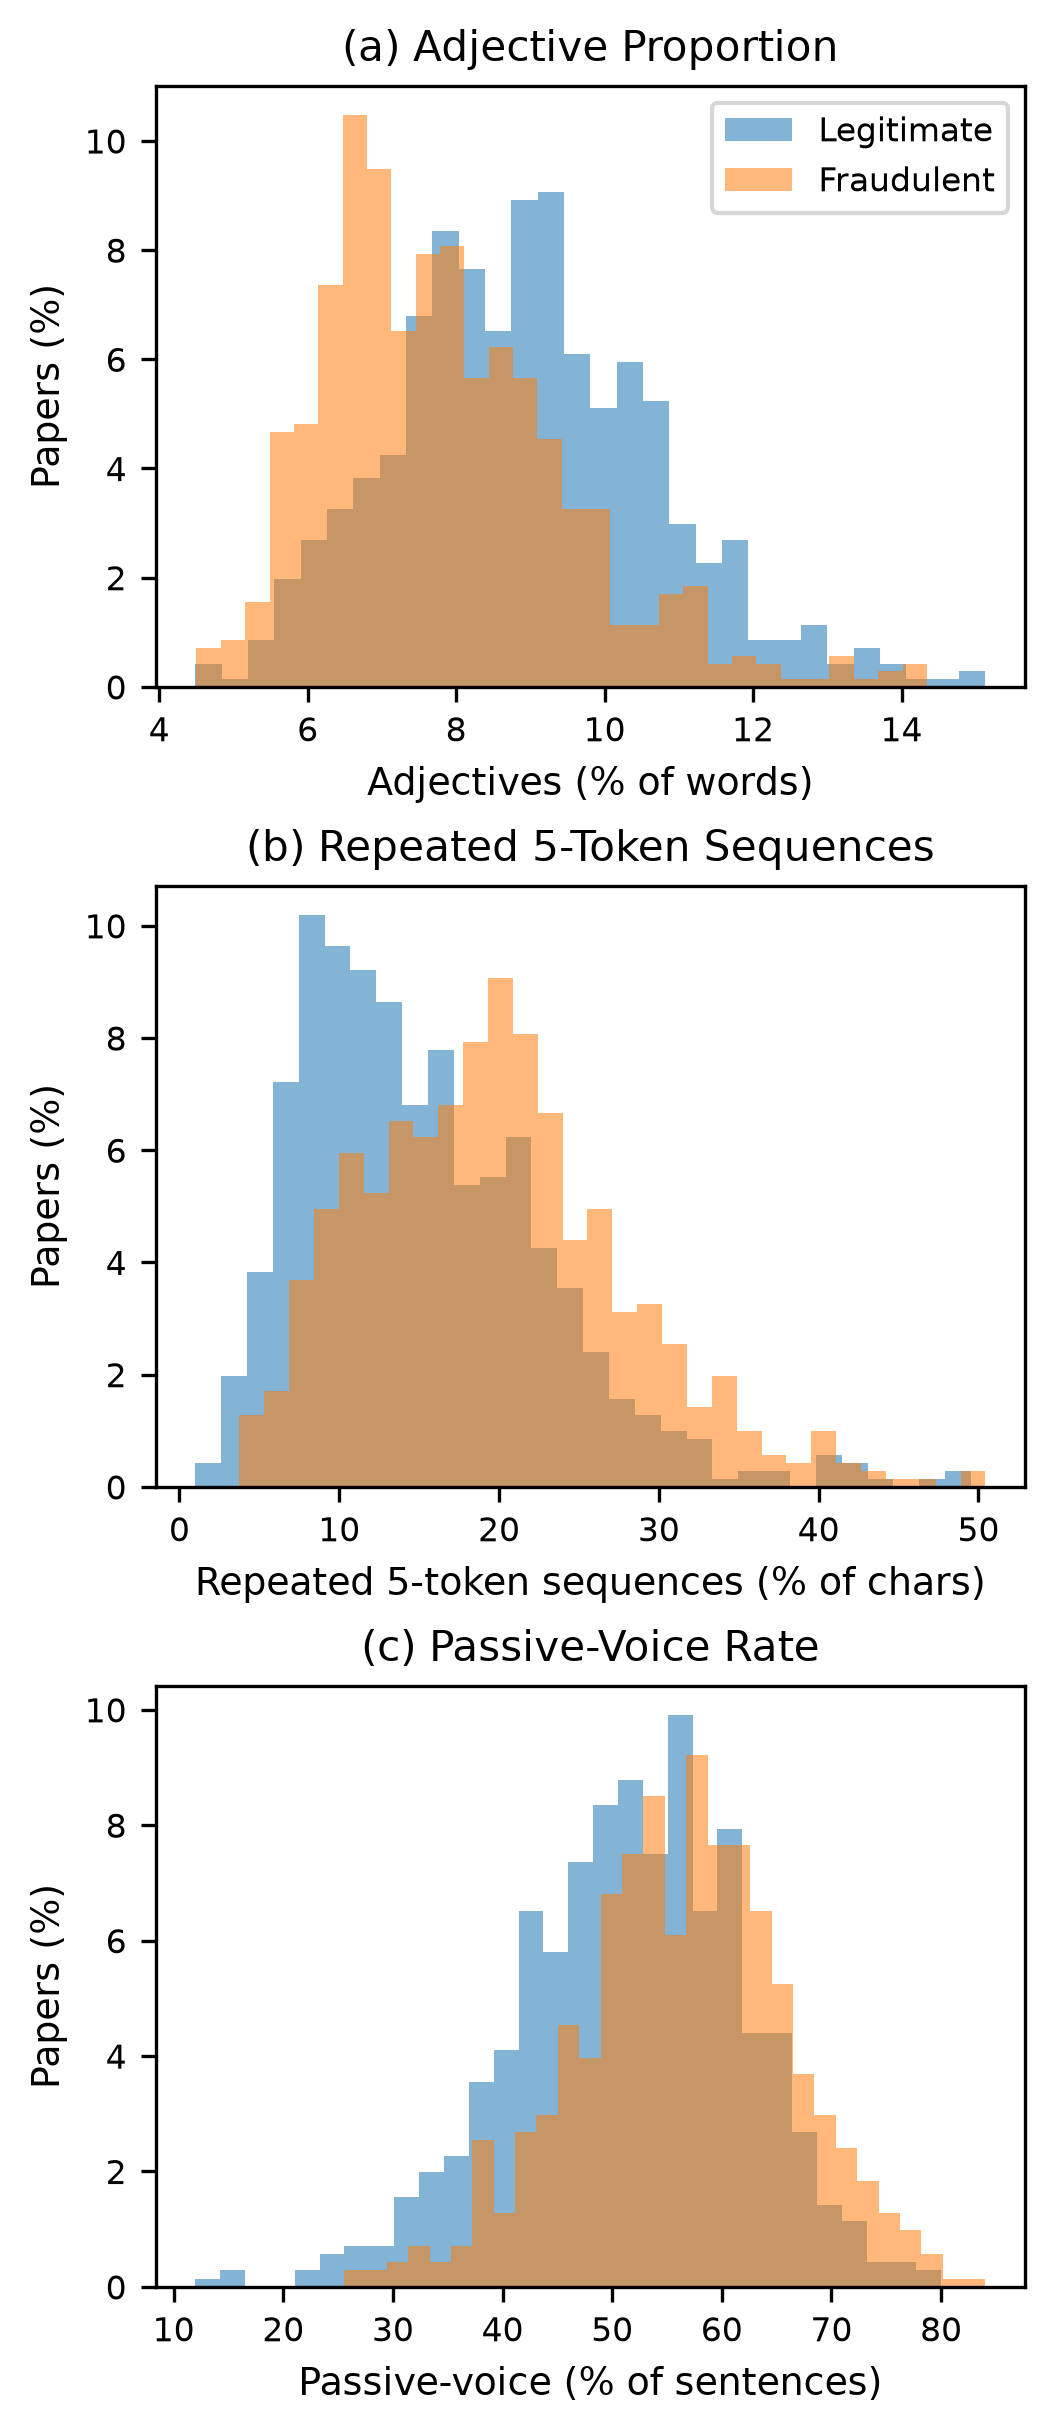
\includegraphics{figures/selected_feature_distributions.png}
    \caption{Distributions of three linguistic features selected to represent the strongest associations distinguishing between the fraudulent and genuine papers. The orange represents the fraudulent papers, and the blue represents the legitimate ones.}
    \label{fig:top-feature-distributions}
\end{figure}

The largest associations with fraud status were observed with the proportions of adjectives ($r=-0.301$) and nouns ($r=0.297$). On average, there are more adjectives and fewer nouns in legitimate papers. Genuine papers also use more modal verbs ($r=-0.224$), negations ($r=-0.197$), determiners ($r=-0.193$), and pronouns ($r=-0.167$). On the other hand, fraudulent papers have more repeated token sequences (for n-grams 5 through 10), passive voice ($r=0.228$),  acronyms ($r=0.178$), and coordinating conjunctions ($r=0.166$).

Adjective proportion, repeated 5-token sequences, and passive voice rate were selected for visualization because they represented the strongest correlations across different feature patterns. Noun proportions were not used due to their close relationship with adjective proportion, and similarly, the other repeated n-token sequence features were not plotted either.

\subsection{Machine Learning Classifier Performance}

The classification performance varied across the four different classifiers and three numerical representations of the paper, as seen in Table 5 below. The highest total accuracy (76.4\%) on the held-out testing dataset was achieved by the RBF SVM model using a combination of both the extracted features and the text embeddings. Using total accuracy was an appropriate way to gauge the performance of the model because the classes are balanced. Regardless, RBF SVM scored the highest on all the standard metrics.

Models trained solely on the linguistic features produced accuracies ranging from 69.4\% to 72.5\%. Accuracy using only text embeddings ranged from 66.5\% to 72.5\%, with the linear models performing worse than the non-linear ones. Similarly, the linear classifiers have lower accuracies when the representations are combined, with accuracies ranging from 67.3\% to 76.4\%.

\begin{table}[H]
\centering
\caption{Confusion matrix for the combined RBF SVM. Percentages are calculated
within each actual class.}
\label{tab:best-confusion-matrix}

\small
\begin{tabular}{lcc}
\toprule
 & \multicolumn{2}{c}{Predicted class} \\
\cmidrule(lr){2-3}
Actual class & Control & Retracted \\
\midrule
Control
    & 102 (71.8\%)
    & 40 (28.2\%) \\

Retracted
    & 27 (19.0\%)
    & 115 (81.0\%) \\
\bottomrule
\end{tabular}
\end{table}

\begin{table*}[t]
\centering
\caption{Classification performance across four classifiers and three article representations as measured by standard metrics. Bold values indicate the best result for each metric.}
\label{tab:model-performance}

\small
\setlength{\tabcolsep}{4.5pt}

\begin{tabular}{llccccc}
\toprule
Representation &
Classifier &
Accuracy &
Precision &
Recall &
F1 &
ROC--AUC \\
\midrule

Linguistic features
    & Logistic regression
    & 72.5 & 70.5 & 77.5 & 73.8 & 0.788 \\

    & Linear SVM
    & 71.1 & 70.0 & 73.9 & 71.9 & 0.790 \\

    & RBF SVM
    & 69.4 & 68.5 & 71.8 & 70.1 & 0.763 \\

    & Random forest
    & 71.8 & 72.1 & 71.1 & 71.6 & 0.767 \\

\addlinespace

Text embeddings
    & Logistic regression
    & 66.5 & 64.4 & 73.9 & 68.9 & 0.739 \\

    & Linear SVM
    & 67.3 & 65.0 & 74.6 & 69.5 & 0.739 \\

    & RBF SVM
    & 72.5 & 69.8 & 79.6 & 74.3 & 0.821 \\

    & Random forest
    & 71.1 & 68.8 & 77.5 & 72.8 & 0.791 \\

\addlinespace

Combined
    & Logistic regression
    & 70.1 & 68.6 & 73.9 & 71.2 & 0.747 \\

    & Linear SVM
    & 67.3 & 65.8 & 71.8 & 68.7 & 0.740 \\

    & RBF SVM
    & \textbf{76.4}
    & \textbf{74.2}
    & \textbf{81.0}
    & \textbf{77.4}
    & \textbf{0.833} \\

    & Random forest
    & 73.6 & 72.8 & 75.4 & 74.0 & 0.790 \\

\bottomrule
\end{tabular}
\end{table*}


The most accurate model, the RBF SVM trained with the combined representations, correctly classified 217 of the 284 papers in the testing set, as seen in the confusion matrix above. The model correctly identified more true positives (81.0\%) than true negatives (71.8\%). Additionally, this model had an F1 score of 77.4\%.

\section{Discussion}

\subsection{Interpretation of Linguistic Features}

Overall, the results support the idea that papers later retracted for fraud-related reasons differ measurably from legitimate papers. Of the 78 retained features, 57 were statistically significant after Benjamini--Hochberg correction. However, the largest correlations were only around 0.30, meaning that no individual feature can be treated as evidence of fraud. Instead, the differences appear to be a collection of small linguistic patterns that become more useful when considered together.

The largest associations were found for adjective and noun proportions. Fraudulent papers used fewer adjectives and more nouns than the controls. The lower adjective proportion agrees with Markowitz and Hancock's 2014 study of Diederik Stapel's papers, which also found fewer adjectives in fraudulent research \cite{markowitz2014}. One possible explanation is that genuine research contains more descriptive detail because the authors are describing experiments and observations that actually occurred. However, adjective usage may also be affected by subject area or journal style. The higher noun proportion may reflect the same overall change in grammatical structure rather than a separate behavior, since all parts-of-speech proportions are calculated from the same collection of words.

Fraudulent papers also used fewer modal verbs. Words such as "may", "might", and "could" are commonly used to qualify findings or express uncertainty. Their lower frequency may suggest that fraudulent findings were presented more confidently. This agrees with previous research finding differences in certainty and hedging language between fraudulent and genuine papers \cite{markowitz2014}.

Passive voice was more common in the fraudulent papers. One possible explanation is that passive language places attention on an action while removing the person performing it. For example, "the samples were analyzed" does not identify the researcher as the actor. This could allow authors to distance themselves from questionable or non-existent procedures. However, passive voice is already extremely common in biomedical writing, especially in Methods sections.

Another major pattern was the greater amount of repeated language in fraudulent papers. All repeated token measures from 5-grams through 10-grams were positively associated with fraud status. This agrees with Bless et al. (2025), who also found greater phrase repetition in retracted papers \cite{bless2025}. Repetition could result from formulaic writing, copied sections, recycled methods, AI-generated text, or templates used by paper mills.

Fraudulent papers also contained more acronyms, which may make the writing more difficult to understand. This could contribute to linguistic obfuscation by making it harder for a reviewer to evaluate the paper closely. 

The citation results did not fully support the original expectation. Fraudulent papers had slightly fewer citation markers per 1,000 words, but the association was very small, and the total number of references did not differ significantly. This contrasts with Markowitz and Hancock (2016), who found that linguistic obfuscation was associated with a greater number of references \cite{markowitz2016}. 

Together, these findings provide some support for the idea of linguistic obfuscation, and clearly demonstrate distinct differences between fraudulent and legitimate papers.

\subsection{Binary Classifier Performance and Comparison with Prior Work}

The best-performing model was the RBF SVM using both the linguistic features and text embeddings. It achieved an accuracy of 76.4\%, an F1 score of 77.4\%, and a ROC--AUC of 0.833. This shows that the language of a paper contains enough information to distinguish the two groups substantially better than chance. However, the model still misclassified 67 of the 284 papers in the testing set, so it cannot independently determine whether a paper is fraudulent.

When only the extracted features were used, the linear models performed relatively well, with logistic regression reaching 72.5\% accuracy. This suggests that some relationships between the features and fraud status could be represented with a relatively simple linear boundary. In contrast, the linear models performed worse with text embeddings, while the non-linear models performed significantly better. Likely, the embeddings contained more complex relationships that RBF SVM and random forest could capture. It then makes sense that combining the features and embeddings improved both nonlinear models but did not improve the linear models.

The model's performance compares favorably with previous research. Markowitz and Hancock's 2014 classifier achieved 71.4\% accuracy, although it used only 49 papers written by one researcher \cite{markowitz2014}. Their later study achieved 57.2\% accuracy with a larger group of authors \cite{markowitz2016}. Braud and S{\o}gaard (2017) achieved approximately 76.0\% accuracy using n-grams and grammatical patterns \cite{braud2017}, which is very similar to the present result, but on a significantly smaller dataset.

This model also outperformed Bless et al. (2025)'s Distributional Quantification Framework, achieving a higher F1 score of 0.774 compared to 0.727 \cite{bless2025}. Unfortunately, the authors did not include any other performance metrics available for comparison.

Overall, the classifier performed very competitively with previous approaches despite using inferior static embeddings and no hyperparameter tuning. The results also suggest that combining interpretable linguistic features with embeddings can improve performance when used with a nonlinear model. This is very notable because this paper's dataset includes both falsification and manipulation of data/images, making this classification a broader and more difficult task, and was done with significantly less computational power.

\subsection{Practical Implications}

The model may be useful as a screening tool for journals or peer reviewers. Its sensitivity of 81.0\% means that it correctly identified 115 of the 142 fraudulent papers in the testing set. Instead of closely investigating every submission, reviewers could use the model to flag papers that may require additional checks, such as image analysis, requests for raw data, or closer statistical review. And having less false negatives (19.0\%) than false positives (28.2\%) is useful because this is a screening tool that should be used by the journals, not the general public. It would be better to review a few extra papers than let possibly fraudulent ones pass without any scrutiny.

However, the model should not be used to accuse an author of misconduct. It incorrectly flagged 40 control papers and missed 27 fraudulent papers. Therefore, its predictions should only be used to prioritize further review, with any final decision based on human judgment and additional evidence.

\subsection{Limitations and Future Directions}

Several limitations should be considered. First, retraction status is an imperfect measure of fraud. Retraction notices may not completely explain what occurred, and not every author may have been responsible. Similarly, the control papers were assumed to be legitimate because they were not known to be retracted. Some may contain undetected problems or may be retracted later.

Second, the dataset only included biomedical papers available in the PubMed Central Open Access Subset. This allowed the full text to be processed consistently, but it limits generalizability to other disciplines and non-open-access publications. Using a different API in the future would allow for larger training and testing sets.

The features and embeddings were also calculated for each paper as a whole. Different sections have different writing styles, such as greater passive-voice usage in Methods and more hedging in Discussions. Future research should analyze paper sections separately rather than averaging them together.

The embedding model was a static, distilled version of PubMedBERT, and all sentence vectors were averaged into one representation. A contextual Transformer fine-tuned on this task may capture more meaning and improve performance. Hyperparameter tuning, feature selection, and probability calibration may also improve the current models.

\section*{Code Availability}

All code, data, and instructions for reproducing the analysis are available at \url{https://github.com/xPugnocode/scientific-fraud-nlp}. The repository also includes instructions for downloading an updated Retraction Watch dataset and running the full analysis pipeline.

\section*{Acknowledgments}

I would like to thank Rachel Hopkins for her guidance, feedback, support, and other mentorship throughout this project.

\bibliography{references}
\bibliographystyle{unsrt}

\clearpage
\appendix

% Required packages:
% \usepackage{booktabs}
% \usepackage{longtable}
% \usepackage{pdflscape}
% \usepackage{array}
% \usepackage[table]{xcolor}

\clearpage
\onecolumn
\begin{landscape}
\scriptsize
\setlength{\tabcolsep}{2.5pt}
\renewcommand{\arraystretch}{1.08}
\setcounter{table}{0}
\renewcommand{\thetable}{\arabic{table}}
\renewcommand{\tablename}{Supplementary Table}


\begin{longtable}{@{}p{5.2cm}p{2.65cm}p{2.65cm}p{2.85cm}p{2.85cm}ccc@{}}
\caption{Complete statistical comparison of the 78 retained handcrafted features, grouped by statistical significance after Benjamini--Hochberg correction.}
\label{tab:supplementary-feature-statistics}\\

\toprule
Feature &
\shortstack{Control\\mean (SD)} &
\shortstack{Retracted\\mean (SD)} &
\shortstack{Control\\median [IQR]} &
\shortstack{Retracted\\median [IQR]} &
$r_{\mathrm{pb}}$ &
$r_{\mathrm{rb}}$ &
BH $q$ \\
\midrule
\endfirsthead

\multicolumn{8}{c}{\tablename\ \thetable{}---continued from previous page}\\
\toprule
Feature &
\shortstack{Control\\mean (SD)} &
\shortstack{Retracted\\mean (SD)} &
\shortstack{Control\\median [IQR]} &
\shortstack{Retracted\\median [IQR]} &
$r_{\mathrm{pb}}$ &
$r_{\mathrm{rb}}$ &
BH $q$ \\
\midrule
\endhead

\midrule
\multicolumn{8}{r}{Continued on next page}\\
\endfoot

\bottomrule
\endlastfoot
\rowcolor{blue!10}
\multicolumn{8}{@{}l}{\textbf{Statistically significant after BH correction ($q < .05$; 57 features)}} \\
\addlinespace[2pt]
Adjective tokens (\% of all tokens) & 8.93 (1.78) & 7.84 (1.68) & 8.89 [7.71--10.05] & 7.64 [6.66--8.79] & $-0.301$ & $-0.526$ & $8.07 \times 10^{-32}$ \\
Noun tokens (\% of all tokens) & 30.87 (2.69) & 32.43 (2.30) & 30.97 [29.19--32.68] & 32.58 [31.03--33.94] & $0.297$ & $0.523$ & $8.23 \times 10^{-32}$ \\
Characters in repeated 5-token sequences (\%) & 15.16 (7.71) & 19.65 (8.11) & 13.79 [9.36--19.95] & 19.23 [13.55--24.21] & $0.273$ & $0.484$ & $1.84 \times 10^{-27}$ \\
Characters in repeated 6-token sequences (\%) & 10.89 (6.80) & 14.63 (7.39) & 9.40 [5.83--14.68] & 13.95 [9.10--18.55] & $0.255$ & $0.465$ & $1.93 \times 10^{-25}$ \\
Characters in repeated 7-token sequences (\%) & 8.21 (6.04) & 11.23 (6.69) & 6.78 [3.74--11.31] & 10.20 [6.32--14.89] & $0.231$ & $0.428$ & $1.02 \times 10^{-21}$ \\
Sentences containing passive voice (\%) & 51.52 (10.49) & 56.27 (9.77) & 52.05 [44.69--58.93] & 56.76 [50.51--62.87] & $0.228$ & $0.380$ & $2.73 \times 10^{-17}$ \\
Modal verbs per 1,000 words & 5.46 (2.70) & 4.30 (2.35) & 5.08 [3.48--6.92] & 3.89 [2.66--5.59] & $-0.224$ & $-0.360$ & $9.76 \times 10^{-16}$ \\
Characters in repeated 8-token sequences (\%) & 6.51 (5.44) & 8.99 (6.08) & 5.12 [2.48--9.04] & 7.73 [4.37--12.33] & $0.211$ & $0.395$ & $1.26 \times 10^{-18}$ \\
Negation dependencies per 1,000 words & 3.86 (2.21) & 3.00 (2.08) & 3.59 [2.17--5.16] & 2.56 [1.50--4.05] & $-0.197$ & $-0.360$ & $9.76 \times 10^{-16}$ \\
Characters in repeated 9-token sequences (\%) & 5.36 (4.95) & 7.47 (5.57) & 3.91 [1.77--7.61] & 6.19 [3.33--10.41] & $0.196$ & $0.369$ & $1.95 \times 10^{-16}$ \\
Determiner tokens (\% of all tokens) & 6.84 (1.74) & 6.20 (1.51) & 6.70 [5.62--7.91] & 5.99 [5.12--7.12] & $-0.193$ & $-0.347$ & $8.58 \times 10^{-15}$ \\
Characters in repeated 10-token sequences (\%) & 4.51 (4.54) & 6.35 (5.14) & 3.16 [1.27--6.49] & 5.18 [2.52--8.81] & $0.187$ & $0.354$ & $3.18 \times 10^{-15}$ \\
Acronym mentions per 1,000 words & 64.66 (34.72) & 76.50 (30.57) & 61.88 [40.74--85.52] & 74.78 [55.30--97.66] & $0.178$ & $0.338$ & $4.40 \times 10^{-14}$ \\
Pronoun tokens (\% of all tokens) & 1.09 (0.51) & 0.94 (0.38) & 0.99 [0.75--1.36] & 0.91 [0.69--1.14] & $-0.167$ & $-0.276$ & $1.02 \times 10^{-9}$ \\
Coordinating-conjunction tokens (\% of all tokens) & 3.53 (0.69) & 3.76 (0.72) & 3.49 [3.07--3.88] & 3.72 [3.29--4.15] & $0.166$ & $0.274$ & $1.42 \times 10^{-9}$ \\
Measure of textual lexical diversity (MTLD) & 83.48 (16.00) & 78.59 (13.13) & 82.58 [71.95--93.20] & 78.12 [69.64--87.52] & $-0.165$ & $-0.249$ & $4.78 \times 10^{-8}$ \\
Unique acronyms with extracted definitions (\%) & 6.34 (6.31) & 4.69 (3.80) & 4.76 [2.44--8.14] & 4.00 [2.18--6.25] & $-0.157$ & $-0.231$ & $5.16 \times 10^{-7}$ \\
Second-order sentence coherence & 0.671 (0.039) & 0.661 (0.035) & 0.670 [0.644--0.697] & 0.660 [0.638--0.680] & $-0.135$ & $-0.235$ & $2.74 \times 10^{-7}$ \\
Segmented type--token ratio & 0.798 (0.024) & 0.792 (0.022) & 0.800 [0.782--0.814] & 0.793 [0.779--0.808] & $-0.135$ & $-0.218$ & $1.58 \times 10^{-6}$ \\
Unique tokens (\% of all tokens) & 27.25 (4.86) & 26.01 (4.60) & 27.17 [23.92--30.46] & 25.75 [22.76--29.08] & $-0.130$ & $-0.246$ & $6.90 \times 10^{-8}$ \\
Verb tokens (\% of all tokens) & 7.70 (1.11) & 7.96 (0.93) & 7.74 [7.01--8.46] & 8.01 [7.35--8.62] & $0.128$ & $0.221$ & $1.25 \times 10^{-6}$ \\
LIX readability index & 62.60 (5.60) & 61.24 (4.92) & 62.05 [58.76--65.22] & 60.93 [57.77--63.91] & $-0.128$ & $-0.219$ & $1.42 \times 10^{-6}$ \\
RIX readability index & 9.68 (1.85) & 9.24 (1.60) & 9.43 [8.41--10.50] & 9.09 [8.12--10.04] & $-0.127$ & $-0.214$ & $2.58 \times 10^{-6}$ \\
Adverb tokens (\% of all tokens) & 2.28 (0.54) & 2.15 (0.51) & 2.23 [1.91--2.61] & 2.10 [1.82--2.43] & $-0.126$ & $-0.220$ & $1.42 \times 10^{-6}$ \\
Sentiment polarity score & 0.0646 (0.0333) & 0.0560 (0.0337) & 0.0643 [0.0444--0.0849] & 0.0558 [0.0361--0.0765] & $-0.126$ & $-0.205$ & $6.44 \times 10^{-6}$ \\
First-order sentence coherence & 0.699 (0.035) & 0.690 (0.032) & 0.699 [0.674--0.721] & 0.689 [0.671--0.708] & $-0.125$ & $-0.228$ & $5.83 \times 10^{-7}$ \\
Hypergeometric distribution diversity (HDD) & 0.869 (0.019) & 0.865 (0.018) & 0.871 [0.858--0.882] & 0.867 [0.854--0.877] & $-0.121$ & $-0.209$ & $3.96 \times 10^{-6}$ \\
Automated Readability Index & 18.81 (2.68) & 18.22 (2.40) & 18.48 [16.96--20.17] & 17.96 [16.55--19.50] & $-0.116$ & $-0.204$ & $6.74 \times 10^{-6}$ \\
Unique acronyms (count) & 71.4 (54.1) & 82.7 (42.4) & 60.5 [36.0--97.8] & 77.0 [54.0--104.0] & $0.116$ & $0.297$ & $5.70 \times 10^{-11}$ \\
Particle tokens (\% of all tokens) & 1.56 (0.43) & 1.47 (0.40) & 1.53 [1.28--1.81] & 1.42 [1.19--1.72] & $-0.115$ & $-0.211$ & $3.53 \times 10^{-6}$ \\
Median sentence length (tokens) & 23.76 (3.38) & 23.03 (3.30) & 23.00 [22.00--26.00] & 23.00 [21.00--25.00] & $-0.109$ & $-0.196$ & $3.64 \times 10^{-5}$ \\
Characters in top 4-token sequences (\%) & 0.71 (0.54) & 0.83 (0.63) & 0.57 [0.36--0.93] & 0.69 [0.42--1.05] & $0.102$ & $0.190$ & $3.11 \times 10^{-5}$ \\
Numeric tokens (\% of all tokens) & 4.12 (1.42) & 3.87 (1.22) & 3.98 [3.23--4.82] & 3.74 [3.03--4.48] & $-0.095$ & $-0.175$ & $1.34 \times 10^{-4}$ \\
Mean sentence length (tokens) & 27.92 (4.58) & 27.09 (4.47) & 27.25 [24.90--30.23] & 26.40 [24.14--29.23] & $-0.092$ & $-0.163$ & $3.77 \times 10^{-4}$ \\
Characters in top 3-token sequences (\%) & 0.93 (0.74) & 1.06 (0.79) & 0.73 [0.41--1.25] & 0.87 [0.49--1.40] & $0.087$ & $0.157$ & $6.27 \times 10^{-4}$ \\
Coleman--Liau Index & 15.92 (1.68) & 15.67 (1.39) & 15.82 [14.83--16.97] & 15.59 [14.75--16.43] & $-0.082$ & $-0.150$ & 0.001 \\
Mean word length (characters) & 4.90 (0.26) & 4.86 (0.22) & 4.89 [4.74--5.06] & 4.85 [4.73--4.99] & $-0.081$ & $-0.162$ & $4.15 \times 10^{-4}$ \\
Hash symbols per 100 words & 0.029 (0.090) & 0.047 (0.146) & 0.000 [0.000--0.000] & 0.000 [0.000--0.021] & $0.074$ & $0.150$ & 0.029 \\
Number-like tokens per 1,000 words & 52.57 (26.78) & 49.18 (17.89) & 49.02 [39.76--61.04] & 47.09 [37.54--57.51] & $-0.074$ & $-0.134$ & 0.004 \\
Sentence-length standard deviation (tokens) & 18.39 (8.50) & 17.28 (6.56) & 16.36 [13.62--20.96] & 15.44 [13.43--18.90] & $-0.073$ & $-0.138$ & 0.003 \\
Mean token length (characters) & 5.58 (0.28) & 5.54 (0.24) & 5.56 [5.39--5.76] & 5.53 [5.38--5.68] & $-0.072$ & $-0.131$ & 0.005 \\
Sentence count & 179.5 (88.9) & 192.1 (87.6) & 159.0 [118.0--219.0] & 181.0 [132.2--232.0] & $0.072$ & $0.178$ & $1.10 \times 10^{-4}$ \\
Gunning Fog Index & 18.76 (2.04) & 18.47 (1.92) & 18.42 [17.43--19.85] & 18.33 [17.08--19.58] & $-0.072$ & $-0.117$ & 0.011 \\
Adposition tokens (\% of all tokens) & 10.79 (1.25) & 10.95 (1.13) & 10.72 [10.03--11.54] & 10.97 [10.26--11.66] & $0.067$ & $0.124$ & 0.007 \\
Flesch--Kincaid Grade Level & 15.13 (1.92) & 14.88 (1.83) & 14.89 [13.85--16.19] & 14.72 [13.59--15.90] & $-0.067$ & $-0.113$ & 0.014 \\
First-person singular pronouns per 1,000 words & 0.55 (1.39) & 0.38 (1.33) & 0.12 [0.00--0.56] & 0.13 [0.00--0.42] & $-0.064$ & $-0.167$ & 0.002 \\
Adjacent dependency relations, sentence-level mean (\%) & 36.48 (0.95) & 36.36 (0.99) & 36.49 [35.88--37.07] & 36.36 [35.69--37.02] & $-0.064$ & $-0.124$ & 0.007 \\
Auxiliary-verb tokens (\% of all tokens) & 3.84 (0.73) & 3.74 (0.69) & 3.80 [3.40--4.33] & 3.72 [3.30--4.15] & $-0.064$ & $-0.133$ & 0.004 \\
SMOG Index & 16.20 (1.33) & 16.05 (1.22) & 16.02 [15.31--17.00] & 15.99 [15.15--16.80] & $-0.058$ & $-0.091$ & 0.049 \\
Punctuation tokens (\% of all tokens) & 14.18 (2.32) & 14.43 (1.98) & 14.12 [12.82--15.39] & 14.43 [13.12--15.61] & $0.058$ & $0.153$ & $8.89 \times 10^{-4}$ \\
Citation markers per 1,000 words & 15.35 (5.98) & 14.71 (5.85) & 14.45 [11.14--18.56] & 13.64 [10.63--17.33] & $-0.055$ & $-0.108$ & 0.018 \\
Token count & 4,890 (2,378) & 5,086 (2,198) & 4,362 [3,319--5,973] & 4,783 [3,672--6,158] & $0.043$ & $0.121$ & 0.008 \\
Document length (quality-component tokens) & 5,758 (2,864) & 5,993 (2,608) & 5,117 [3,860--7,020] & 5,624 [4,338--7,267] & $0.043$ & $0.125$ & 0.007 \\
Character count & 27,980 (13,192) & 29,015 (12,343) & 25,058 [19,368--34,292] & 27,238 [21,001--35,253] & $0.041$ & $0.109$ & 0.017 \\
Syllables-per-token standard deviation & 1.08 (0.17) & 1.10 (0.19) & 1.06 [1.01--1.11] & 1.07 [1.03--1.12] & $0.040$ & $0.120$ & 0.009 \\
Entropy score & 142.6 (72.2) & 147.2 (64.2) & 125.6 [96.1--173.4] & 138.3 [106.3--178.3] & $0.033$ & $0.116$ & 0.011 \\
Token-length standard deviation (characters) & 4.20 (2.68) & 4.03 (3.32) & 3.63 [3.44--4.06] & 3.61 [3.44--3.88] & $-0.027$ & $-0.130$ & 0.005 \\
\addlinespace[4pt]
\midrule
\rowcolor{gray!18}
\multicolumn{8}{@{}l}{\textbf{Not statistically significant after BH correction ($q \geq .05$; 21 features)}} \\
\addlinespace[2pt]
\rowcolor{gray!7}
Mean syllables per token & 1.68 (0.08) & 1.69 (0.07) & 1.68 [1.63--1.73] & 1.69 [1.64--1.73] & $0.044$ & $0.068$ & 0.150 \\
\rowcolor{gray!7}
Median token length (characters) & 4.62 (0.50) & 4.58 (0.49) & 5.00 [4.00--5.00] & 5.00 [4.00--5.00] & $-0.037$ & $-0.087$ & 0.169 \\
\rowcolor{gray!7}
Subordinating-conjunction tokens (\% of all tokens) & 0.87 (0.33) & 0.89 (0.32) & 0.83 [0.65--1.04] & 0.87 [0.67--1.07] & $0.036$ & $0.074$ & 0.118 \\
\rowcolor{gray!7}
Proper-noun tokens (\% of all tokens) & 2.58 (1.09) & 2.52 (1.01) & 2.44 [1.75--3.19] & 2.39 [1.80--3.12] & $-0.029$ & $-0.051$ & 0.278 \\
\rowcolor{gray!7}
First-person plural pronouns per 1,000 words & 5.86 (3.89) & 5.64 (3.65) & 5.54 [2.86--8.22] & 5.36 [2.86--7.56] & $-0.028$ & $-0.066$ & 0.161 \\
\rowcolor{gray!7}
Mean dependency distance & 3.56 (0.27) & 3.55 (0.28) & 3.54 [3.41--3.70] & 3.52 [3.39--3.69] & $-0.027$ & $-0.057$ & 0.226 \\
\rowcolor{gray!7}
Median syllables per token & 1.00 (0.00) & 1.00 (0.04) & 1.00 [1.00--1.00] & 1.00 [1.00--1.00] & $0.027$ & $1.000$ & 1.000 \\
\rowcolor{gray!7}
Alphabetic-word count & 4,238 (2,021) & 4,338 (1,844) & 3,750 [2,919--5,143] & 4,012 [3,142--5,216] & $0.026$ & $0.081$ & 0.084 \\
\rowcolor{gray!7}
Flesch Reading Ease & 36.32 (7.54) & 36.64 (6.88) & 36.78 [31.97--41.40] & 37.17 [32.68--41.37] & $0.022$ & $0.029$ & 0.573 \\
\rowcolor{gray!7}
Other/unknown tokens (\% of all tokens) & 0.765 (0.801) & 0.796 (0.800) & 0.472 [0.281--0.874] & 0.513 [0.298--0.960] & $0.020$ & $0.060$ & 0.204 \\
\rowcolor{gray!7}
Sentiment subjectivity score & 0.432 (0.042) & 0.430 (0.041) & 0.431 [0.407--0.460] & 0.431 [0.403--0.455] & $-0.020$ & $-0.038$ & 0.433 \\
\rowcolor{gray!7}
Interjection tokens (\% of all tokens) & 0.0101 (0.0202) & 0.0093 (0.0261) & 0.0000 [0.0000--0.0148] & 0.0000 [0.0000--0.0111] & $-0.018$ & $-0.108$ & 0.097 \\
\rowcolor{gray!7}
Tokens containing alphabetic characters (\%) & 80.73 (3.59) & 80.85 (2.99) & 81.14 [78.87--82.94] & 81.05 [79.30--82.68] & $0.018$ & $0.016$ & 0.765 \\
\rowcolor{gray!7}
Stop-word count & 1,767 (866) & 1,793 (780) & 1,566 [1,194--2,123] & 1,659 [1,275--2,170] & $0.016$ & $0.067$ & 0.159 \\
\rowcolor{gray!7}
Dependency-distance standard deviation & 1.23 (0.64) & 1.22 (0.51) & 1.14 [0.99--1.31] & 1.12 [1.00--1.31] & $-0.015$ & $0.018$ & 0.728 \\
\rowcolor{gray!7}
Symbol tokens (\% of all tokens) & 0.048 (0.119) & 0.045 (0.117) & 0.010 [0.000--0.050] & 0.007 [0.000--0.042] & $-0.011$ & $-0.025$ & 0.695 \\
\rowcolor{gray!7}
Acronyms with extracted definitions (count) & 3.58 (2.91) & 3.53 (2.62) & 3.00 [2.00--5.00] & 3.00 [2.00--5.00] & $-0.008$ & $0.002$ & 0.984 \\
\rowcolor{gray!7}
Adjacent dependency relations, sentence-level SD (\%) & 5.67 (0.70) & 5.66 (0.65) & 5.62 [5.22--6.00] & 5.59 [5.20--6.01] & $-0.008$ & $-0.020$ & 0.708 \\
\rowcolor{gray!7}
Characters in top 2-token sequences (\%) & 1.03 (0.91) & 1.02 (0.82) & 0.81 [0.42--1.24] & 0.80 [0.43--1.28] & $-0.005$ & $-0.004$ & 0.968 \\
\rowcolor{gray!7}
Unique-token count & 1,248 (414) & 1,245 (359) & 1,187 [983--1,455] & 1,220 [1,000--1,430] & $-0.004$ & $-0.003$ & 0.981 \\
\rowcolor{gray!7}
Out-of-vocabulary words (\%) & 3.89 (1.72) & 3.88 (1.69) & 3.65 [2.57--4.81] & 3.55 [2.71--4.58] & $-0.002$ & $0.002$ & 0.981 \\
\end{longtable}

\begin{minipage}{\linewidth}
\footnotesize
\textit{Note.} Features are grouped by statistical significance after Benjamini--Hochberg correction and ordered within each group by descending absolute point-biserial correlation with retraction status. Light gray shading indicates non-significant results ($q \geq .05$). 
SD, standard deviation; IQR, interquartile range; $r_{\mathrm{pb}}$, point-biserial correlation; $r_{\mathrm{rb}}$, rank-biserial correlation; BH $q$, Benjamini--Hochberg-adjusted $p$-value from the paired two-sided Wilcoxon signed-rank test. The analysis included 706 matched pairs. Positive correlations indicate higher values among retracted articles; negative correlations indicate higher values among control articles.
\end{minipage}

\end{landscape}
\clearpage
\twocolumn


\end{document}
